%!TEX program = xelatex
% 完整编译: xelatex -> biber/bibtex -> xelatex -> xelatex
\documentclass[lang=cn,11pt,a4paper]{elegantpaper}

\title{curvature.h说明文档}
\author{Haochen Huang}
\institute{西安交通大学MFM课题组}

\version{0.02}
\date{\zhtoday}

% 本文档命令
\usepackage{array}

\begin{document}

\maketitle
\begin{abstract}
  本文为curvature.h文件的说明文档,该头文件为工具类型的头文件,基于height.h所计算出的界面高度值,提供求解相应界面网格上的曲率值的工具,为tension.h,contact.h,reduced.h等头文件提供所需函数。本头文件共分为两个部分:网格单元所含曲率求解以及界面网格势能求解。本版本为\textbf{草稿},三种求解方式中的height函数值拟合与直接拟合由于需要parabola.h中的相关函数,暂时搁置,在完成parabola.h相应文档编写后再行增补。
\end{abstract}

\tableofcontents

\section{网格单元曲率求解}
本章内容共分为两个部分:三种曲率求解方式以及相应网格单元上曲率的综合计算,其中三种求解方式为之后的曲率综合计算提供相应的工具,而最终的求解则是依照具体情况选择适当的方法对相应网格进行计算。\par
本章共分为三个小节,按照程序编写顺序,第一章简介曲率在树状网格下的细分和合并,第二章具体讲解三种曲率计算函数,第三章则是汇总讲解曲率控制函数,介绍单元网格上的曲率是如何分步骤被计算确定的。
\subsection{曲率在树状网格下的细分合并}
注意两个函数中的判断对象,当所有子单元中\mintinline{lexer.py:DiffLexer -x}{kappa[] == nodata}时判断进入否定,取值\mintinline{lexer.py:DiffLexer -x}{nodata} 
\begin{minted}[mathescape=true,breaklines]{lexer.py:DiffLexer -x}
/**
# Curvature of an interface

The curvature field is defined only in interfacial cells. In all the
other cells it takes the value *nodata*. 

On trees, we need to redefine the restriction function to take
this into account i.e. the curvature of the parent cell is the average
of the curvatures in the interfacial child cells. */

#if TREE
static void curvature_restriction (Point point, scalar kappa)
{
  double k = 0., s = 0.;
  foreach_child()
    if (kappa[] != nodata)
      k += kappa[], s++;
  kappa[] = s ? k/s : nodata;//注意这里的判断并不是kappa[]==s,而是直接判断s值是否为0,如果是0则说明子单元中没有任何的界面单元,若不是0则该单元则继承子单元中边界单元的平均曲率
}

/**
The prolongation function performs a similar averaging, but using the
same stencil as that used for bilinear interpolation, so that the
symmetries of the volume fraction field and curvature field are
preserved. */

static void curvature_prolongation (Point point, scalar kappa)
{
  foreach_child() {
    double sk = 0., s = 0.;
    for (int i = 0; i <= 1; i++)
    #if dimension > 1
      for (int j = 0; j <= 1; j++)
    #endif
      #if dimension > 2
  for (int k = 0; k <= 1; k++)
      #endif
  if (coarse(kappa,child.x*i,child.y*j,child.z*k) != nodata)
    sk += coarse(kappa,child.x*i,child.y*j,child.z*k), s++;
    kappa[] = s ? sk/s : nodata;
  }
}
#endif // TREE
\end{minted}
\subsection{三种曲率计算函数}
首先介绍利用"height.h"函数直接通过定义式计算曲率的方法,再获得相应坐标高度后曲率计算如下(二维/三维)
\begin{align}
  \kappa &= \frac{h_{xx}}{(1 + h_x^2)^{3/2}}\\
  \kappa &= \frac{h_{xx}(1 + h_y^2) + h_{yy}(1 + h_x^2) - 2h_{xy}h_xh_y}{(1 + h_x^2 + h_y^2)^{3/2}}
\end{align}
相应函数总体可分为两部分:即曲率、法向量计算函数 \mintinline{lexer.py:DiffLexer -x}{kappa(), normal()},以及综合函数 \mintinline{lexer.py:DiffLexer -x}{height_curvature()},首先来介绍两个功能函数。\par  
在这里需要注意两个问题,首先由于曲率计算方法不同,2维与3维相关工具函数依靠宏定义被区分开,其次需要注意Basilisk中自带的宏工具\mintinline{lexer.py:DiffLexer -x}{foreach_dimension},该工具会在编译阶段将带有"$\_x,.x$"的代码块复制,并依照"$(x,y,z)$"的顺序进行递进,下文中出现的定义的函数例如 \mintinline{lexer.py:DiffLexer -x}{kappa_z()}在3D情况下编译时会自动生成函数 \mintinline{lexer.py:DiffLexer -x}{kappa_y(),kappa_x()},相关高度生成部分请参看"height.h说明文档" 
\begin{minted}[mathescape=true,breaklines]{lexer.py:DiffLexer -x}
/**
## Height-function curvature and normal


The normal is computed in a similar way, but also allowing for
asymmetric 2-points stencils and taking into account the
orientation. */

#include "heights.h"

#if dimension == 2
foreach_dimension()//foreach_dimension为basilisk自定义的指令,在程序编译时该指令会将作用范围内所有的代码进行复制,并将表示下标的函数、参数进行遍历如“.x,.y”以及“_x, _y”,也就是说下文中的kappa_y函数在实际的编译过程中被复制成为了两个函数(宏定义为二维环境)kappa_x, 以及kappa_y
static double kappa_y (Point point, vector h)
{
  int ori = orientation(h.y[]);//orientation 函数用来鉴定该网格高度的法方向
  for (int i = -1; i <= 1; i++)
    if (h.y[i] == nodata || orientation(h.y[i]) != ori)//如果在周围网格内有height为nodata或者相邻网格height方向不相符合的情况,就将该网格的曲率定义为nodata
      return nodata;
  double hx = (h.y[1] - h.y[-1])/2.;
  double hxx = (h.y[1] + h.y[-1] - 2.*h.y[])/Delta;
  return hxx/pow(1. + sq(hx), 3/2.);//直接做二阶精度的差分进行相关计算
}

foreach_dimension()//basilisk中所有的坐标在只有单坐标时例如h.x[i],其所对应的指标为x轴
static coord normal_y (Point point, vector h)
{
  coord n = {nodata, nodata, nodata};
  if (h.y[] == nodata)
    return n;
  int ori = orientation(h.y[]);
  if (h.y[-1] != nodata && orientation(h.y[-1]) == ori) {
    if (h.y[1] != nodata && orientation(h.y[1]) == ori)//同样的确定相应网格的height值1.同方向 2.不是nodata
      n.x = (h.y[-1] - h.y[1])/2.;
    else
      n.x = h.y[-1] - h.y[];//边界处理,当h.y[1]不存在时取一阶精度
  }
  else if (h.y[1] != nodata && orientation(h.y[1]) == ori)
    n.x = h.y[] - h.y[1];//同理,取一阶精度
  else
    return n;
  double nn = (ori ? -1. : 1.)*sqrt(1. + sq(n.x));//如此做法的原因就是因为高度函数在非沿界面方向上,相邻两个单元网格的height之差还就是1,详情见height.h
  n.x /= nn;
  n.y = 1./nn;//将法向量的两个分量进行单位化
  return n;
}//同一个网格会由两个方向的高度函数拟合出两个相对应的法向量
#else // dimension == 3
foreach_dimension()//三维情况下的曲率计算,同理该函数在实际编译时被复制成为3份,分别是kappa_x,kappa_y,kappa_z
static double kappa_z (Point point, vector h)
{
  int ori = orientation(h.z[]);
  for (int i = -1; i <= 1; i++)
    for (int j = -1; j <= 1; j++)
      if (h.z[i,j] == nodata || orientation(h.z[i,j]) != ori)
  return nodata;
  double hx = (h.z[1] - h.z[-1])/2.;
  double hy = (h.z[0,1] - h.z[0,-1])/2.;

  /**
  We "filter" the curvature using a weighted sum of the three
  second-derivatives in the $x$ and $y$ directions. This is necessary
  to avoid a numerical mode when the curvature is used to compute
  surface tension. */
  
  double filter = 0.2;
  double hxx = (filter*(h.z[1,1] + h.z[-1,1] - 2.*h.z[0,1]) +
    (h.z[1] + h.z[-1] - 2.*h.z[]) +
    filter*(h.z[1,-1] + h.z[-1,-1] - 2.*h.z[0,-1]))//在此处需要强调的是这里的z轴坐标全部都默认为当前位置,在该z坐标下进行一个平面上的高度函数二阶导数相关计算
    ((1. + 2.*filter)*Delta);
  double hyy = (filter*(h.z[1,1] + h.z[1,-1] - 2.*h.z[1]) +
    (h.z[0,1] + h.z[0,-1] - 2.*h.z[]) +
    filter*(h.z[-1,1] + h.z[-1,-1] - 2.*h.z[-1]))/
    ((1. + 2.*filter)*Delta);
  double hxy = (h.z[1,1] + h.z[-1,-1] - h.z[1,-1] - h.z[-1,1])/(4.*Delta);
  return (hxx*(1. + sq(hy)) + hyy*(1. + sq(hx)) - 2.*hxy*hx*hy)/
    pow(1. + sq(hx) + sq(hy), 3/2.);
}//foreach_dimension的具体操作其实质上就是转换坐标,在保持右手坐标系的前提下遍历每个方向上的坐标可能性

foreach_dimension()
static coord normal2_z (Point point, vector h)
{
  scalar hz = h.z;
  if (hz[] == nodata)
    return (coord){nodata, nodata, nodata};
  int ori = orientation(hz[]);
  double a = ori ? -1. : 1.;
  coord n;
  n.z = a;
  foreach_dimension(2) {//在此处foreach_dimension后跟2代表在x方向和y方向上进行循环遍历,请注意,此时函数方向为“_z”在进入别的方向判定时,该循环就是在相应坐标下的x,y方向循环了
    if (allocated(-1) && hz[-1] != nodata && orientation(hz[-1]) == ori) {//allocate函数具体操作内容未知
      if (allocated(1) && hz[1] != nodata && orientation(hz[1]) == ori)
        n.x = a*(hz[-1] - hz[1])/2.;
      else
        n.x = a*(hz[-1] - hz[]);//进入该循环说明在某一方向上height函数无法取值,此时取一阶精度
    }
    else if (allocated(1) && hz[1] != nodata && orientation(hz[1]) == ori)//与上同理
      n.x = a*(hz[] - hz[1]);
    else
      n.x = nodata;
  }
  return n;
}

foreach_dimension()
static coord normal_z (Point point, vector h) {
  coord n = normal2_z (point, h);//调用之前定义的函数,其中z方向的值应该为1
  double nn = fabs(n.x) + fabs(n.y) + fabs(n.z);
  if (nn < nodata) {
    foreach_dimension()
      n.x /= nn;//将相应的法向量单位化
    return n;
  }
  return (coord){nodata, nodata, nodata};//如果相应的值中有nodata的存在返回nodata向量
}
#endif
\end{minted}
接下来介绍综合函数 \mintinline{lexer.py:DiffLexer -x}{height_curvature(), height_normal()}在前文中通过相应的宏工具生成了计算各个方向曲率以及法向量的工具函数,这一组函数的功能就是在前文函数的基础上决定使用哪一个方向计算曲率法向量并进行保存 
\begin{minted}[mathescape=true,breaklines]{lexer.py:DiffLexer -x}
/**
We now need to choose one of the $x$, $y$ or $z$ height functions to
compute the curvature. This is done by the function below which
returns the HF curvature given a volume fraction field *c* and a
height function field *h*. */

static double height_curvature (Point point, scalar c, vector h)
{

  /**
  We first define pairs of normal coordinates *n* (computed by simple
  differencing of *c*) and corresponding HF curvature function *kappa*
  (defined above). */

  typedef struct {
    double n;
    double (* kappa) (Point, vector);
  } NormKappa;
  struct { NormKappa x, y, z; } n; //定义命名为n的结构体,其内容包含三个命名为x y z的MNormKappa结构体 
  foreach_dimension()
    n.x.n = c[1] - c[-1], n.x.kappa = kappa_x;//将相关结构体名下的函数变量指向之前定义的函数kappa_x(在上一小节中定义了三个函数kappa_x, kappa_y, kappa_z)
  double (* kappaf) (Point, vector) = NULL; NOT_UNUSED (kappaf);//定义一个同类型数据的空指针
  
  /**
  We sort these pairs in decreasing order of $|n|$. */
  
  if (fabs(n.x.n) < fabs(n.y.n))
    swap (NormKappa, n.x, n.y);//注意swap的功能是进行内存地址的相互交换,也就是说交换后排在第一个位置的值依旧是n.x只不过相应的指向内容变成原本n.y的内存内容,也就是说在n.x下储存的函数名有可能是kappa_y
#if dimension == 3
  if (fabs(n.x.n) < fabs(n.z.n))
    swap (NormKappa, n.x, n.z);
  if (fabs(n.y.n) < fabs(n.z.n))
    swap (NormKappa, n.y, n.z);
#endif

  /**
  We try each curvature function in turn. */

  double kappa = nodata;//从相应fraction变化最剧烈的地方开始进行计算
  foreach_dimension()
    if (kappa == nodata) {
      kappa = n.x.kappa (point, h);
      if (kappa != nodata) {//如果kappa已经赋值成功,那么就跳过对kappa的相应赋值,将原本的数据结构重新指向上文中定义好的kappa类型空指针中
        kappaf = n.x.kappa;
        if (n.x.n < 0.)
          kappa = - kappa;//若体积分数移动方向为递减,则相应的曲率应当是负数值
      }
    }

  if (kappa != nodata) {
    
    /**
     We limit the maximum curvature to $1/\Delta$. */

    if (fabs(kappa) > 1./Delta)
      kappa = sign(kappa)/Delta;
    
    /**
     We add the axisymmetric curvature if necessary. */
      
#if AXI//旋转对称相关,具体内容待查
    double nr, r = y, hx;
    if (kappaf == kappa_x) {
      hx = (height(h.x[0,1]) - height(h.x[0,-1]))/2.;
      nr = hx*(orientation(h.x[]) ? 1 : -1);
    }
    else {
      r += height(h.y[])*Delta;
      hx = (height(h.y[1,0]) - height(h.y[-1,0]))/2.;
      nr = orientation(h.y[]) ? -1 : 1;
    }
    /* limit the minimum radius to half the grid size */
    kappa += nr/max (sqrt(1. + sq(hx))*r, Delta/2.);
#endif
  }
  
  return kappa;
}

/**
The function below works in a similar manner to return the normal
estimated using height-functions (or a *nodata* vector if this cannot
be done). */

coord height_normal (Point point, scalar c, vector h)
{

  /**
  We first define pairs of normal coordinates *n* (computed by simple
  differencing of *c*) and corresponding normal function *normal*
  (defined above). */

  typedef struct {
    double n;
    coord (* normal) (Point, vector);
  } NormNormal;
  struct { NormNormal x, y, z; } n;//与上一个函数同等,对相应结构体赋值函数  
  foreach_dimension()
    n.x.n = c[1] - c[-1], n.x.normal = normal_x;
  
  /**
  We sort these pairs in decreasing order of $|n|$. */
  
  if (fabs(n.x.n) < fabs(n.y.n))
    swap (NormNormal, n.x, n.y);
#if dimension == 3
  if (fabs(n.x.n) < fabs(n.z.n))
    swap (NormNormal, n.x, n.z);
  if (fabs(n.y.n) < fabs(n.z.n))
    swap (NormNormal, n.y, n.z);
#endif

  /**
  We try each normal function in turn. */

  coord normal = {nodata, nodata, nodata};
  foreach_dimension()
    if (normal.x == nodata)
      normal = n.x.normal (point, h);
  
  return normal;//相应的nodata选项已经在normal函数中被排除掉了
}

/**
In three dimensions, these functions return the (two) components of
the normal projected onto the $(x,y)$ plane (respectively). */

#if dimension == 3
foreach_dimension()//此函数具体的功能待查,目前并没有遇见任何头文件中带有本函数
coord height_normal_z (Point point, vector h)
{
  coord nx = normal2_x (point, h);
  coord ny = normal2_y (point, h);
  if (fabs(nx.y) < fabs(ny.x)) {
    normalize (&nx);
    return nx;
  }
  else if (ny.x != nodata) {
    normalize (&ny);
    return ny;
  }
  return (coord){nodata, nodata, nodata};
}
#endif
\end{minted}
\subsection{曲率综合计算}
接下来介绍一个单元网格内的曲率是如何被计算完成的,按照程序编写顺序,首先介绍边界判断函数,该函数返回bool值,用于判断网格是否处于边界上或其相邻单元网格是否是边界(如果该单元的相邻单元是边界单元,那么也需要对其进行赋值,用于曲率拟合、平均等)
\begin{minted}[mathescape=true,breaklines]{lexer.py:DiffLexer -x}
/**
## General curvature computation

We first need to define "interfacial cells" i.e. cells which contain
an interface. A simple test would just be that the volume fraction is
neither zero nor one. As usual things are more complicated because of
round-off errors. They can cause the interface to be exactly aligned
with cell boundaries, so that cells on either side of this interface
have fractions exactly equal to zero or one. The function below takes
this into account. */

static inline bool interfacial (Point point, scalar c)
{
  if (c[] >= 1.) {
    for (int i = -1; i <= 1; i += 2)
      foreach_dimension()
        if (c[i] <= 0.)//只要有一个方向上的体积分数值越过界面为零,那么就认为该网格就是界面网格
          return true;
  }
  else if (c[] <= 0.) {
    for (int i = -1; i <= 1; i += 2)
      foreach_dimension()
        if (c[i] >= 1.)
          return true;
  }
  else // c[] > 0. && c[] < 1.
    return true;
  return false;
}//该函数的创建目的就是为了防止界面与网格界面完全重合,导致并没有网格体积分数在0,1之间但依旧是界面网格
\end{minted}
接下来介绍曲率计算的整体控制函数。曲率计算流程如下
\begin{figure}[h]
    \centering
    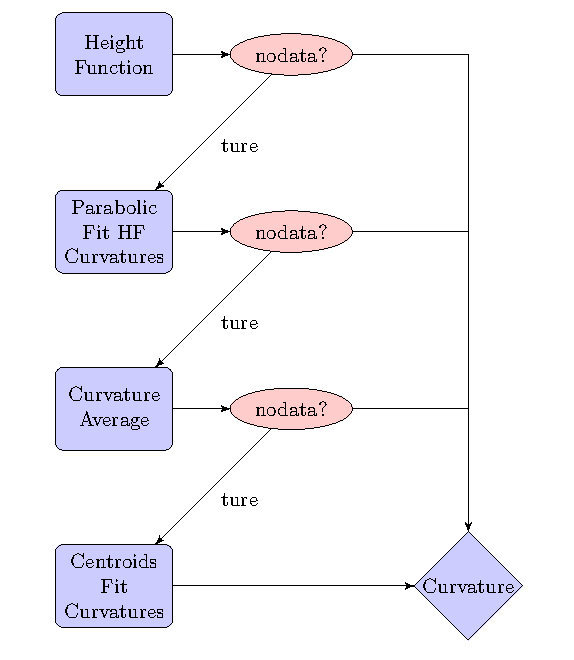
\includegraphics[width=0.5\textwidth]{image/workflow2.pdf}
    \caption{曲率整体计算流程}
\end{figure}
\begin{minted}[mathescape=true,breaklines]{lexer.py:DiffLexer -x}
/**
The function below computes the mean curvature *kappa* of the
interface defined by the volume fraction *c*. It uses a combination of
the methods above: statistics on the number of curvatures computed
which each method is returned in a *cstats* data structure. 

If *sigma* is different from zero the curvature is multiplied by *sigma*.

If *add* is *true*, the curvature (optionally multiplied by *sigma*)
is added to field *kappa*. */

typedef struct {
  int h; // number of standard HF curvatures
  int f; // number of parabolic fit HF curvatures
  int a; // number of averaged curvatures
  int c; // number of centroids fit curvatures
} cstats;

struct Curvature {
  scalar c, kappa;
  double sigma;
  bool add;
};

trace
cstats curvature (struct Curvature p)
{
  scalar c = p.c, kappa = p.kappa;
  double sigma = p.sigma ? p.sigma : 1.;
  int sh = 0, sf = 0, sa = 0, sc = 0;
  vector ch = c.height, h = automatic (ch);
  if (!ch.x.i)
    heights (c, h);

  /**
  On trees we set the prolongation and restriction functions for
  the curvature. */
  
#if TREE
  kappa.refine = kappa.prolongation = curvature_prolongation;
  kappa.restriction = curvature_restriction;
#endif

  /**
  We first compute a temporary curvature *k*: a "clone" of
  $\kappa$. */
  
  scalar k[];
  scalar_clone (k, kappa);

  foreach(reduction(+:sh) reduction(+:sf)) {

    /**
    If we are not in an interfacial cell, we set $\kappa$ to *nodata*. */

    if (!interfacial (point, c))
      k[] = nodata;

    /**
    Otherwise we try the standard HF curvature calculation first, and
    the "mixed heights" HF curvature second. */ 
    
    else if ((k[] = height_curvature (point, c, h)) != nodata)//也就意味着有且仅有界面单元才会被赋予曲率,否则不会有相应的kappa值
      sh++;
    else if ((k[] = height_curvature_fit (point, c, h)) != nodata)//直接使用曲率计算公式计算失败,转为使用height函数值进行拟合
      sf++;
  }
  
  foreach (reduction(+:sa) reduction(+:sc)) {
    
    /**
    We then construct the final curvature field using either the
    computed temporary curvature... */

    double kf;
    if (k[] < nodata)//已经计算出kappa了
      kf = k[];
    else if (interfacial (point, c)) {//进入该循环的条件就是即没有曲率值,但是又存在于界面上,那就说明上一个函数中的两种曲率计算已经失败了

      /**
      ...or the average of the curvatures in the $3^{d}$ neighborhood
      of interfacial cells. */
      
      double sk = 0., a = 0.;
      foreach_neighbor(1)//循环遍历每个方向正负的网格单位
        if (k[] < nodata)
          sk += k[], a++;
      if (a > 0.)//如果周围有网格成功通过计算得出了相应的曲率值,那么就直接取相应网格上的曲率平均
        kf = sk/a, sa++;
      else

	/**
	Empty neighborhood: we try centroids as a last resort. */

        kf = centroids_curvature_fit (point, c), sc++;//而如果连周围网格都没有曲率计算成功,那么就只能使用网格中心拟合了
    }
    else
      kf = nodata;

    /**
    We add or set *kappa*. */
    
    if (kf == nodata)
      kappa[] = nodata;
    else if (p.add)
      kappa[] += sigma*kf;
    else
      kappa[] = sigma*kf;      
  }

  return (cstats){sh, sf, sa, sc};//返回量是cstats型数据,其中包含用不同方式计算曲率的网格个数,sh直接定义计算(最高精度),sf通过height值进行拟合,sa通过周围网格进行平均,sc直接通过周边网格的不同相含量
}
\end{minted}

\section{边界单元势能求解}
本章介绍函数的目的是求解方程
\begin{equation}\label{equ:po}
  \mathbf{G} \cdot ( \mathbf{x} - \mathbf{Z})
\end{equation}
其中$ \mathbf{G}$为自定义势能常数向量(例如重力加速度)$ \mathbf{x}, \mathbf{Z}$分别为边界单元位置坐标与零势能座标点。下文中定义的所有函数均在"reduced.h"中被引用,相关用法请见"reduced.h说明文档"\par
本章同样分为两小节,分别是相应的工具函数以及整体的势能求解,其代码中的大部分逻辑与前文相类似,故不再赘述。
\subsection{势能求解工具函数}
本小节分为两部分,与曲率求解类似,首先是直接求解方程\ref{equ:po}的工具函数\mintinline{lexer.py:DiffLexer -x}{pos_x},由于求解的对象为边界单元,为了提高求解的精度需要在0势能面垂直方向上增加边界高度即$height$,由此第二个函数的目的就是仿照曲率计算的选择方法,选择相应的法方向累加边界厚度。 
\begin{minted}[mathescape=true,breaklines]{lexer.py:DiffLexer -x}
//注意以下部分函数的调用位置为“reduced.h”,具体作用是使用势场来定义加速度,而不是寻常的直接重写acceleration event
/**
# Position of an interface

with $\mathbf{G}$ and $\mathbf{Z}$ two vectors and $\mathbf{x}$ the
coordinates of the interface.

This is defined only in interfacial cells. In all the other cells it
takes the value *nodata*.

We first need a function to compute the position $\mathbf{x}$ of an
interface. For accuracy, we first try to use height functions. */

foreach_dimension()
static double pos_x (Point point, vector h, coord * G, coord * Z)
{
  if (fabs(height(h.x[])) > 1.)//注意fabs(height(h.x[]))>1.会将一部分界面网格过滤,见说明
    return nodata;
  coord o = {x, y, z};//在此处直接定义了该网格所处的坐标位置
  o.x += height(h.x[])*Delta;//由于过滤掉了非界面网格,此处的作用就是精确的定义界面所在的相关位置
  double pos = 0.;
  foreach_dimension()//注意这里foreach_dimension()相关操作目的是进行矢量点乘
    pos += (o.x - Z->x)*G->x;
  return pos;//根据矢量计算返回pos值
}

/**
We now need to choose one of the $x$, $y$ or $z$ height functions to
compute the position. This is done by the function below which returns
the HF position given a volume fraction field *f*, a height function
field *h* and vectors *G* and *Z*. */

static double height_position (Point point, scalar f, vector h,
coord * G, coord * Z)
{

  /**
  We first define pairs of normal coordinates *n* (computed by simple
  differencing of *f*) and corresponding HF position function *pos*
  (defined above). */

  typedef struct {
    double n;
    double (* pos) (Point, vector, coord *, coord *);
  } NormPos;//定义一种NormPos数据类型
  struct { NormPos x, y, z; } n;//n中包含三个NormPos类型的数据
  foreach_dimension()
    n.x.n = f[1] - f[-1], n.x.pos = pos_x;//注意,此处是一个函数指针传递,也就是说该位置寄存的应该是上文中定义的pos_x函数
  
  /**
  We sort these pairs in decreasing order of $|n|$. */
  
  if (fabs(n.x.n) < fabs(n.y.n))
    swap (NormPos, n.x, n.y);
#if dimension == 3
  if (fabs(n.x.n) < fabs(n.z.n))
    swap (NormPos, n.x, n.z);
  if (fabs(n.y.n) < fabs(n.z.n))
    swap (NormPos, n.y, n.z);
#endif

  /**
  We try each position function in turn. */
  //老方法,尝试直接返回$\mathbf{G}(\mathbf{x}-\mathbf{Z})$
  double pos = nodata;
  foreach_dimension()
    if (pos == nodata)
      pos = n.x.pos (point, h, G, Z);

  return pos;
}
\end{minted}
\subsection{势能综合计算函数}
在此处需要注意的是,之前的工具函数\mintinline{lexer.py:DiffLexer -x}{pos_x}中对于边界网格的筛选是不完全的(例如"height.h说明文档"图5),所以在本函数中对\textbf{是边界网格,但是height(h.x[])>1}的网格进行基于$f$的高度拟合(类似于曲率计算中的centroids fit curvatures) 
\begin{minted}[mathescape=true,breaklines]{lexer.py:DiffLexer -x}
/**

If *add* is *true*, the position is added to *pos*. */

struct Position {
  scalar f, pos;//注意在这里pos已经是场量了
  coord G, Z;
  bool add;
};

void position (struct Position p)
{
  scalar f = p.f, pos = p.pos;//最终的计算结果将会添加到pos中
  coord * G = &p.G, * Z = &p.Z;//注意这里均是对地址的操作,在之后的代码中任何对f、pos的操作都是直接对结构体p中的相关项进行赋值操作

  /**
  On trees we set the prolongation and restriction functions for
  the position. */
  
#if TREE
  pos.refine = pos.prolongation = curvature_prolongation;
  pos.restriction = curvature_restriction;
#endif

  vector fh = f.height, h = automatic (fh);
  if (!fh.x.i)
    heights (f, h);
  foreach() {
    if (interfacial (point, f)) {//如果网格是边界网格则进入该判断
      double hp = height_position (point, f, h, G, Z);
      if (hp == nodata) {//进入该循环则意味着该网格是界面网格但fabs(height(h.x[])) > 1.

/**
If the height function is not defined, we use the centroid of
the reconstructed VOF interface. */

        coord n = mycs (point, f), o = {x,y,z}, c;//这里是定义一个数据类型为coord的n并在之后使用函数对其进行赋值
        double alpha = plane_alpha (f[], n);
        plane_area_center (n, alpha, &c);
        hp = 0.;
        foreach_dimension()
          hp += (o.x + Delta*c.x - Z->x)*G->x;
      }
      if (p.add)//决定是否在原有网格值上进行相加还是直接覆盖
        pos[] += hp;
      else
        pos[] = hp;
    }
    else
      pos[] = nodata;
  }
}
\end{minted}

\end{document}
